%%%%%%%%%%%%%%%%%%%%%%%%%%%%%%%%%%%%%%%%%%%%%%%%%%%%%%%%%%%%%%%%%%%%
% This is a thesis template for Gebze Technical University.
%
% Please only edit the areas proceeded by a comment starting with %%
% otherwise the template may be broken.
%
% This file is only to be used for editing the general fields
% and inputting the body of the thesis in the designated areas.
% Please write the body of the thesis in separate files, and input
% them as shown in the comment preceding the area.
%
% Created in Aug 2021 by Usama Derbashi.
%%%%%%%%%%%%%%%%%%%%%%%%%%%%%%%%%%%%%%%%%%%%%%%%%%%%%%%%%%%%%%%%%%%%
\documentclass[12pt]{report}


% Language and typeset setting
\usepackage[english]{babel}
\usepackage[a4paper,top=25mm,bottom=25mm,left=40mm,right=25mm]{geometry}
\usepackage[onehalfspacing]{setspace}
\usepackage{algorithm, algpseudocode}
\usepackage{indentfirst}
\setlength{\parindent}{1cm}
\setlength{\abovecaptionskip}{12pt plus 0pt minus 0pt}
\setlength{\belowcaptionskip}{12pt plus 0pt minus 0pt}
\setlength{\textfloatsep}{18.0pt plus 0.0pt minus 0.0pt}
\setlength{\floatsep}{18.0pt plus 0.0pt minus 0.0pt}
\setlength{\intextsep}{18.0pt plus 0.0pt minus 0.0pt}
\setlength{\skip\footins}{18.0pt plus 0.0pt minus 0.0pt}

% Core packages and settings
\usepackage[colorlinks=false]{hyperref}
\usepackage{amsmath}

\usepackage{titlesec} %setting the titles of chapters and sections
\setcounter{secnumdepth}{4}
\setcounter{tocdepth}{4}
\titleformat{\chapter}[hang]{\normalfont\bfseries\MakeUppercase}{}{0pt}{\LARGE\thechapter. }
\titleformat{\section}[hang]{\normalfont\bfseries}{}{0pt}{\Large\thesection. }
\titleformat{\subsection}[hang]{\normalfont\bfseries}{}{0pt}{\large\thesubsection. }
\titleformat{\subsubsection}[hang]{\normalfont\bfseries}{}{0pt}{\large\thesubsubsection. }
\titlespacing*{\chapter}{0pt}{0pt}{18pt}
\titlespacing*{\section}{0pt}{18pt}{18pt}
\titlespacing*{\subsection}{0pt}{18pt}{18pt}
\titlespacing*{\subsubsection}{0pt}{18pt}{18pt}

\usepackage{graphicx}
\graphicspath{{./Imgs/}} %pointing the directory of images

\usepackage{fancyhdr} % setting footers
\usepackage{etoolbox} 
\renewcommand{\headrulewidth}{0pt}
\patchcmd{\chapter}{\thispagestyle{plain}}{\thispagestyle{fancy}}{}{}
\pagestyle{fancy}
\fancyhf{}
\fancyfoot[C]{\fontsize{11pt}{11pt}\thepage}

\usepackage[style=ieee]{biblatex}
\addbibresource{refs.bib}
\usepackage{csquotes}% Needed for babel(in biblatex)

\usepackage[bottom, perpage]{footmisc}%% amkes footnotes at the bottom

\usepackage{GTUThesis}


% Additional packages if needed
%% For the sake of not messing the template add them here
\usepackage{lipsum}


% Important information
%% Make sure to enter all the info below
\title{Static Overflow Analysis and Tests}
\author{Tugay Apaydın}
\faculty{Faculty of Engineering}
\department{Computer Engineering Department}
\supervisor{Prof. İbrahim SOĞUKPINAR}
\theyear{2022}


\begin{document}

%Front Matter
\pagenumbering{roman} %start with roman numbering 
\projecttitlepageenglish
\maketitle
\setcounter{page}{3} %the first two title pages are not counted so this is a buffer
\begin{outertitles} % makes titles centred

%% below enter as follows 
%% {DATE_OF_DEMO}{JURY}
%% Note that JURY should be comma separated
\makejury{31/08/2021}{Prof. Erchan Aptoula, M.Sc Melike Ilteralp}
%\chapter*{Abstract}
\addcontentsline{toc}{chapter}{Abstract}

%% Edit below this line
Lorem Ipsum is simply dummy text of the printing and typesetting industry. Lorem Ipsum has been the industry's standard dummy text ever since the 1500s, when an unknown printer took a galley of type and scrambled it to make a type specimen book. It has survived not only five centuries, but also the leap into electronic typesetting, remaining essentially unchanged. It was popularised in the 1960s with the release of Letraset sheets containing Lorem Ipsum passages, and more recently with desktop publishing software like Aldus PageMaker including versions of Lorem Ipsum.

%% Until here
\vfill
%% Edit after {Keywords:}
\textbf{Keywords:} keyword1, keyword2.
\clearpage
\chapter*{Özet}
\addcontentsline{toc}{chapter}{Özet}

%% Edit below this line
This study presents a static analysis tool for C language that can detect some buffer overflows that are generally called integer and stack overflows. Buffer overflows occur when a program tries to access to outside of an allocated memory area. In most cases, this causes the program to crash. In a worse scenario, a buffer overflow can provide the access an attacker needs to gain remote code execution. To provide secure code against buffer overflows, programmers need methods for analyzing source code of a program to detect buffer overflow vulnerabilities. One way to implement such a method is to perform static analysis on the program. This involves looking at the source code to find the errors in the program. This study uses syntax analysis and then value flow analysis to find overflows in a source code of a program.

%% Until here
\vfill
%% Edit after {Anahtar Kelimeler:}
%\textbf{Anahtar Kelimeler:} anahtar kelime1, anahtar kelime2.
\clearpage
%\chapter*{Acknowledgement}
\addcontentsline{toc}{chapter}{Acknowledgement}

%% Edit below this line
Thank you mate!!



%% Until here
\vspace{1cm}
\begin{flushright}
\textbf{Name Surname} %% your name here
\end{flushright}
\clearpage
%\chapter*{List of Symbols and Abbreviations}
\addcontentsline{toc}{chapter}{List of Symbols and Abbreviations}

\begin{tabular}{lcl}
    \textbf{Symbol or}&&\\
    \textbf{Abbreviation} &:& \textbf{Explanation}\\
    
    %% Edit below in the format
    %% XYZ &:& EXPLANATION\\
    %% where XYZ is the acronym or symbol
    %% and EXPLANATION is the explanation of it
    %% make sure not to forget &:& between them, and \\ at the end of EXPLANATION
    
    ABC &:& The first three letters in the English alphabet\\
    $\mu$ &:& Small mu\\
    
    %% Until here
\end{tabular}

\clearpage

\tableofcontents
\addcontentsline{toc}{chapter}{Contents}
\clearpage

\listoffigures
\addcontentsline{toc}{chapter}{List of Figures}
\clearpage

\listoftables
\addcontentsline{toc}{chapter}{List of Tables}
\clearpage

\end{outertitles}
\fancyhf{}%reset footer
\fancyfoot[R]{\fontsize{11pt}{11pt}\thepage}%page numbers in the corner
\addtocontents{toc}{\protect\vspace{18pt}}
\pagenumbering{arabic}%turn to arabic numbers

% Mainmatter

%% Only input files, don't write here
%% \input{./Body/Mainmatter/FILE}
\chapter{INTRODUCTION}
\section{PROBLEM DEFINITION}

Buffer overflows are common vulnerabilities in software. In the languages that offer direct, low-level access to read and write memory such as C and C++, buffer overflow vulnerabilities deal with buffers or memory allocations. In the best cases, this type of access causes the program to crash. In the worst case, a buffer overflow can be exploited to hijack control of a program.

The attacks caused by buffer overflow continue to be the major computer security threats. As a traditional exploit, buffer overflow allows attackers to inject malicious codes in the application at run-time. Those injected codes can help attacker to gain the access privilege of the host machine maliciously.

Even though buffer overflow has been intensively studied and researchers have proposed various mitigation techniques, it is still the most critical security threat these days. According to statistics from CERT Coordination Center, the number of identified and catalogued vulnerabilities has increased over 213\% in years between 2004-2006 as shown in Figure \ref{fig:1}.

\begin{figure}[!htbp]
    \centering
    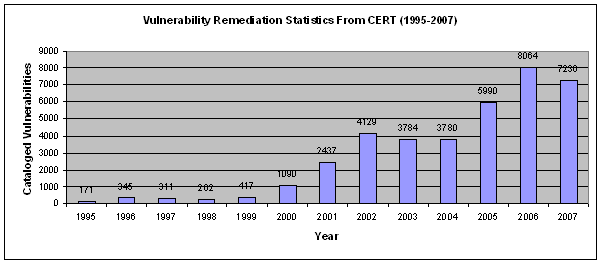
\includegraphics[width=0.8\textwidth]{Imgs/1.png}
    \caption{\label{fig:1} The Catalogued Vulnerabilities Data from CERT Coordination Center from 1995 to 2007  \cite{One}.}
\end{figure}
Due to its importance, researchers have proposed various approaches to defend against buffer overflow attacks. However, each of them has its own limitations and cannot be applied universally to prevent overflow attacks. 

In this project, it is aimed to detect and test buffer overflow vulnerabilities in a source code using static analysis techniques. \cite{Two}


\section{MOTIVATION}
Being able to detect overflows would improve software assurance. Static analysis can be used as a baseline for determining the susceptibility of a program to cause buffer overflows.  

When a new buffer overflow vulnerability is first exploited, a primary challenge is to diagnose the vulnerability. The diagnosis results include which buffer was overflowed; under what conditions the buffer will be overflowed. 

This research investigates the viability of a buffer overflow detection method to statically analyse source files for buffer overflows. The research focuses on the discovery of stack-based, heap-based and integer overflows that occur in C programs.
\chapter{RELATED STUDY}

The aim of software security is that software continues to function correctly even while under attack. Memory errors do not always expose a way for an attacker to exploit them but even in these cases an attacker could potentially exploit these problems in order to perform a very effective denial of service attack. However, when memory errors in programs exposed to the internet are exploitable, they can lead to the attackers gaining control over an entire systems. So from a safety viewpoint it is also very important to make sure these types of errors are found and fixed. Or mitigated some other way, for example with dynamic checks around memory access. This means that not using static analysis may make software much more vulnerable to attacks, than if a static analysis tool was used that can detect various issues.

C and languages similar to it employ manual memory management. These types of languages are not memory safe languages as they require the programmer to explicitly request and free memory when needed instead of the language taking care of it automatically. C and C++ are examples of these kind of, memory unsafe languages. 

The most common issues, in not memory safe languages, are array bounds checking problems (buffer overflow and underflow), not releasing memory (memory leak), releasing memory too soon (also called dangling pointers), and problems with using uninitialized data. 

This study aims to create a static analysis tool for detecting buffer overflow vulnerabilities.

\section{STATIC ANALYSIS APPROACH}
Sophisticated techniques couple static code analysis with formal methods. Formal methods apply theoretical computer science fundamentals to solve difficult problems in software, such as proving that the software will not fail with a run-time error. The combination of static code analysis and formal methods enables developers to detect difficult to find errors and prove the absence of certain types of bugs/errors. E.g. these techniques can prove that the following line of code will never fail with a divide by zero run-time error. Most of today’s tools for static analysis function in basically the same way. They receive code as input, build a model that represents the program, perform some sort of analysis in combination with knowledge about what to search for and finally present the result to the user. Figure \ref{fig:st_analyse} shows the process that all static analysis tools that target security make use of.

\clearpage

\begin{figure}[!htbp]
    \centering
    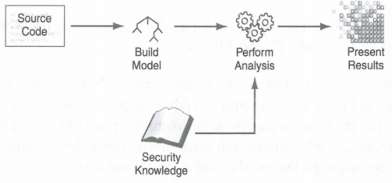
\includegraphics[width=0.8\textwidth]{Imgs/st_analyse.png}
    \caption{\label{fig:st_analyse} Generalized view of the process of a static analysis}
\end{figure}


The first step taken by the tools when performing an analysis is to build a model of the program. In this way an abstract representation of the program is created, which is better suited to be used for the actual analysis and what kind of model that is created depends largely on what kind of analysis that is to be performed. The simplest model, used in a lexical analysis, is a stream of tokens. This is created by taking the source code first. Then discarding all unimportant features such as white spaces and comments and finally translates all parts of the code into tokens.

This stream can then be used to perform a simple lexical analysis on. The next step is to translate the stream of tokens into a parse tree by using a parser that matches the token stream against a set of production rules. The parse tree contains the most direct representation of the code just as the programmer wrote it and can thus be used as a good base to perform analysis.

However, since the production rules might intro duce various symbols in order to make the parsing easy, a parse tree is not the best representation to perform more complex analyzes on. The next step is instead to translate the parse tree into an AST as well as creating a symbol table alongside it. These can then be used as input to a semantic analysis of the program. Another thing that the AST might be used for is to scan it by using predefined patterns in order to find errors that require data-flow analysis of the code. This is not possible to perform on for example a token stream. The procedure of performing a static analysis is until now very alike the procedure taken by a compiler when compiling a program.

But as a compiler as a next step will use the AST to generate an intermediate representation of the code, which can be used for optimization and later on translation to platform specific code, the processes now separates. Most of the tools instead continue by building a control flow graph, which can be used to inspect the various paths in the program or to track data flow, on top of the AST. The way the graph is used by a tool depends largely on which techniques the tool makes use of and this has a big impact on efficiency, speed and result of a scan.

Another thing that influences the result of a scan is how the tool makes certain simplifications of the program. The very essence of a static analyzer is that the program being analyzed is not run. However, in order to perform a through scan the tool, as already described, translates the code into an abstract representation and then “executes” the program on an abstract machine with a set of non-standard values replacing the standard ones. This is where a concept referred to as states is introduced. States are a collection of program variables and the association of values to those variables. 

For every program statement the state of a variable may change in some way and the aim for a static analysis is to associate the set of all possible states with all program points. 

The use of states and how a tool makes the approximations and the simplified descriptions of sets is something that makes the tools differs greatly from one and another. Some make very sophisticated and accurate decisions in order not to make unjustified assumptions about the result of an operation whilst others resort to a more simple approach. This incremental approach goes against what almost everyone in the industry tries to do, especially with security. As the code is being developed, it needs to be brought under the security policy, quality policy, whatever in every single day. If they keep on top of it, it hardly impacts the team’s workflow at all. In fact, it actually saves them time when you factor in the benefits of the error prevention it delivers. But if they allow it to lapse, catching up becomes too overwhelming. \cite{Five}

\section{EXISTING BUFFER OVERFLOW DETECTION METHODS}
\subsection{ARCHER (Array Checker)}
ARCHER is a constraint solver tool that checks the bounds of the variables and memory
sizes of various objects. ARCHER statically analyzes the source code for memory constraint violations such as array accesses, pointer dereferences, or calls to a function that expects a size parameter.

\subsection{BOON (Buffer Overrun Detection)}
BOON was developed to detect buffer overflows using integer range analysis. This is achieved by parsing through the program looking for string variables. When found, string variables are assigned two integers. The first integer is the string’s allocated size, and the second is the number of bytes currently in use. Then, the algorithm checks the usage of each string to determine if the length of the string is greater than the size allocated for the string.

\subsection{UNO (Uninitialized Variables, Nil-Pointer Dereferencing, And Out of Bound Array Indexing)}
In other buffer overflow detection techniques, false positives are common. UNO is a tool that aims to reduce the number of false positive reported and to allow users to define their own application-dependent properties for checking for flaws. As its name indicates, the tool checks for errors such as uninitialized variables, nil-pointer dereferencing, and out of bound array indexing. UNO is an extension of a tool called ctree, which produces a parse tree of a program. UNO runs the ctree program to get a parse tree, then converts the tree into a control flow graph. Once the graph is created, UNO performs its buffer overflow analysis on the control flow graph. Overall, UNO requires two passes through the code. The first pass is to build the tree and graph, and then check for errors.

\subsection{Value Set Analysis}
Value set analysis is the technique of recovering “information about the contents of machine registers and memory locations at every program point in an executable”. This technique was used by Kindermann to perform buffer overflow detection via the static analysis 7 of executables. This buffer overflow detection method focused on the detection of buffer overflows caused by loops.
\cite{Four}.
\chapter{PROJECT DESIGN}
\section{INTRODUCTION}

Many different buffer overflow attacks use different strategies and target different
pieces of code. Below are the best-known buffer overflow vulnerabilities:\\
Types of buffer overflows:\\
•	Stack Overflow\\
•	Heap Overflow\\
•	Integer Overflow\\
•	Unicode Overflow\\

The design of this program will include static analysis of Integer and Stack based overflows.

\begin{figure}[!htbp]
    \centering
    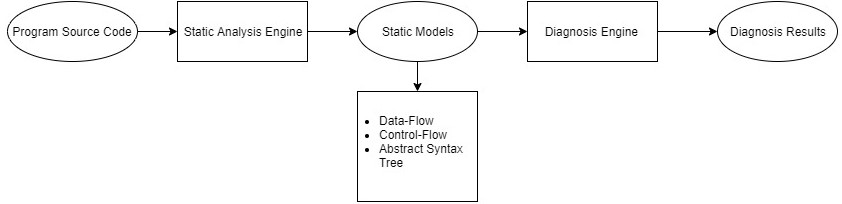
\includegraphics[width=1\textwidth]{Imgs/static_analysis.jpg}
    \caption{\label{fig:SysArch}System Architecture}
\end{figure}

The static analysis engine builds models by parsing the source code of the computer software and creates static models. The models are consist of abstract syntax trees.

The diagnosis engine analysis the models created by static analysis engine. By using the analysis results, it creates results of potential overflows. 

\section{STATIC ANALYSIS ENGINE}
The static analysis engine firstly parses the source code into tokens. After that, it creates abstract syntax tree by analysing statements and expressions. In this project, statements and expressions are limited with some types such as if statements, assign statements and while loops. Also data types are limited with primitive int and char types. Also stack arrays and pointers can be parsed by static analysis engine.

\begin{figure}[!htbp]
    \centering
    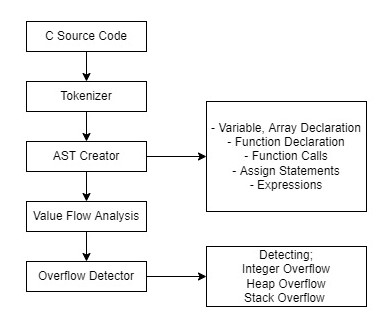
\includegraphics[width=0.8\textwidth]{Imgs/Structure.jpg}
    \caption{\label{fig:SysArch}System Architecture}
\end{figure}

\section{DIAGNOSIS ENGINE}
The diagnosis engine starts with value flow analysis. The statements inside the abstract syntax tree are executed at first. 

While this execution in progress, the overflow check occurs. For example, the expressions are tested before the execution if any overflow may occur. Also, array bound check and other type of buffer overflows are checked in this step.
\subsubsection{Integer Overflow Analysis}
In the design of the project, each expression are designed to return a result. And while calculating the result of the statements, overflow conditions may occur. That's why, at each result calculation, integer overflow analysis is done. 

The integer overflow in a program that is written with C language results in undefined behaviour. That's why, the overflow analysis is done before the statement executions or before calculating expression results.

\begin{figure}[!htbp]
    \centering
    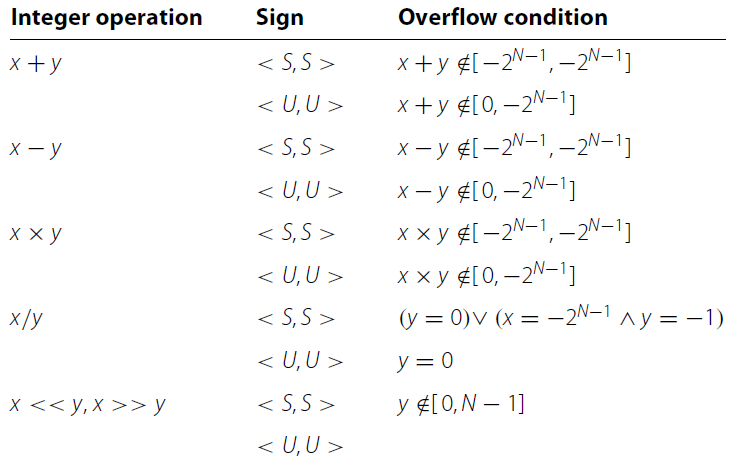
\includegraphics[width=0.8\textwidth]{Imgs/Integer_Overflow_conditions.png}
    \caption{\label{fig:SysArch}Integer Overflow Conditions}
\end{figure}

The figure 2.3 shows the overflow condition for integer operations. \cite{Three}

\subsubsection{Stack and Heap Overflow Analysis}
Stack and heap overflows are caused by accessing outside the bounds of the allocated area. That's why, the bound checking is the first criteria for stack and heap overflow analysis.

There are many unsafe Standard C Library and system data copy functions that can cause buffer overflow vulnerabilities. By using static analysis, it is not possible to detect overflows without analysing the source code. 

\begin{figure}[!htbp]
    \centering
    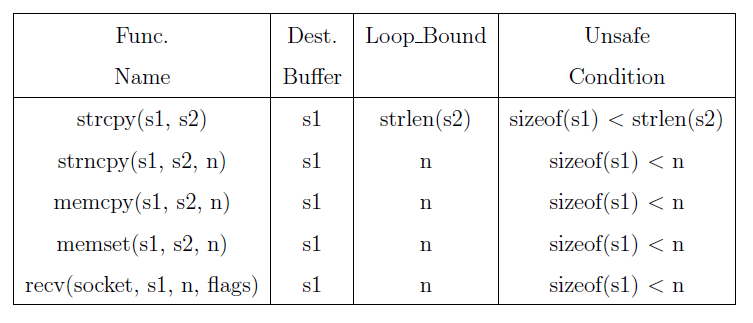
\includegraphics[width=0.8\textwidth]{Imgs/unsafefuncs.png}
    \caption{\label{fig:SysArch}The sample unsafe standard C library functions \cite{One}}
\end{figure}

In the figure 2.4, some sample of vulnerable standard C library functions are listed. The static analysis tools must be aware of these type of functions and analyse their parameters to detect buffer overflows.

\begin{figure}[!htbp]
    \centering
    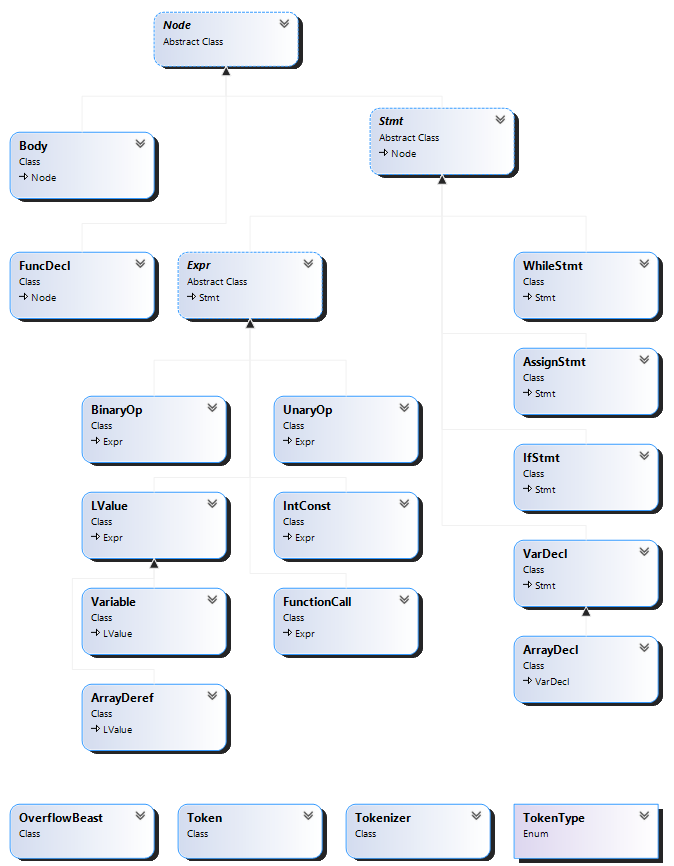
\includegraphics[width=1\textwidth]{Imgs/ClassDiagram2.png}
    \caption{\label{fig:ClassDiagram}Class Diagram}
\end{figure}

\clearpage

\section{REQUIREMENTS}

The project requirements are listed below:
\begin{itemize}
    \item The program shall be able to detect integer, stack and heap based overflow vulnerabilities.
    \item The program shall be able to detect overflows caused by vulnerable C library functions.
    \item The program will list errors in a Graphical User Interface.
    \item C# Language and libraries.
    \item Static analysis tools such as CppCheck for tests and comparisons.
    \item Microsoft Visual Studio IDE for creating GUI and developing the program.
    

\end{itemize}
\chapter{IMPLEMENTATION AND TESTS}
First of all, in this project only several syntax and statement models are implemented in the given time. That's why, the tests and experiments are limited.

In the test file, there are some integer overflows, an array bound overflow (which occurs when trying to access outside of an allocated area) and a stack-heap based overflow which occurs in a vulnerable C library function strcpy(). Figure \ref{fig:TestCode} shows the test code.

\begin{figure}[!htbp]
    \centering
    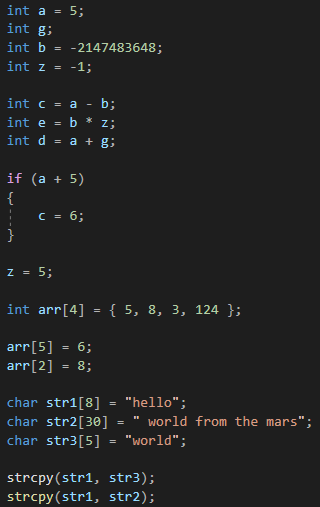
\includegraphics[width=0.4\textwidth]{Imgs/test_code2.png}
    \caption{\label{fig:TestCode} The test file}
\end{figure}

In figure \ref{fig:TestResult}, the overflow analysis of our program showed in graphical user interface.

In figure \ref{fig:TestResult}, the overflow analysis results of our program are showed in a user interface.

\clearpage

\begin{figure}[!htbp]
    \centering
    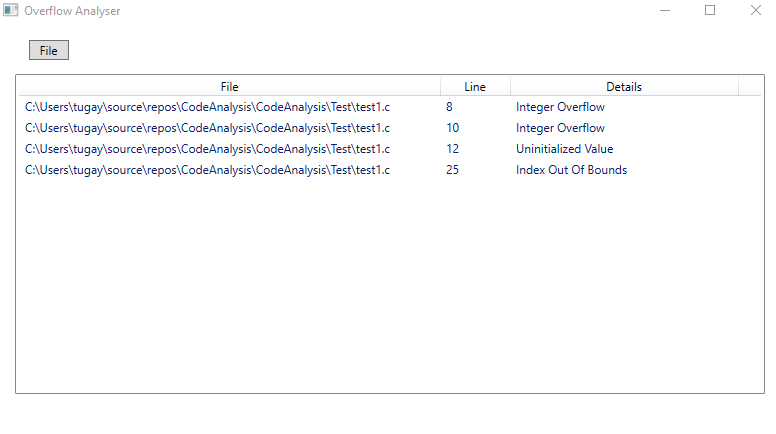
\includegraphics[width=0.7\textwidth]{Imgs/test_result.png}
    \caption{\label{fig:TestResult} An example result list from the GUI}
\end{figure}

In figure \ref{fig:TestCppResult} the same test file is analysed with CppCheck program. It can be seen that the only difference is the overflow that occurs in strcpy() function. 

\begin{figure}[!htbp]
    \centering
    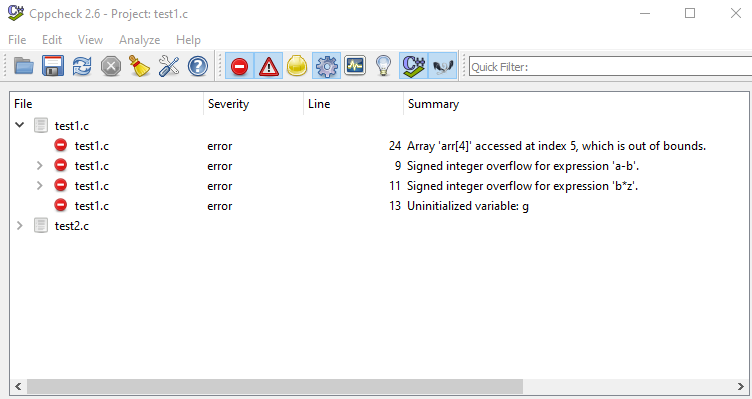
\includegraphics[width=0.8\textwidth]{Imgs/cppcheck_test.png}
    \caption{\label{fig:TestCppResult} CppCheck Results}
\end{figure}

There are many vulnerable C library functions that can cause overflows. But, static analysis can only be done on source code. That's why, static analysis has some disadvantages. In this condition, I manually defined vulnerable C library functions. That's why, my program was able to detect overflow caused at strcpy() function call.
\chapter{CONCLUSION}
In this project, some integer and stack based overflow conditions are handled. The integer overflows for expressions and bound limits for stack arrays are checked. As a result, the possible problems are list using a GUI. 

The program generally creates a syntax representation of the source code. After that, it performs value flow analysis to detect overflows. Currently, the syntax of the C language is very limited. After detecting the overflows, the errors are listed in the GUI.

In future study, the syntax analyser implemented in this project should be improved. The expression and statement models should cover all C Language syntax models. The diagnosis engine also modified according to syntax analyser. 

% DON'T INPUT FILES AFTER HERE
\begin{outertitles}
\clearpage
\setlength{\emergencystretch}{1em}
\printbibliography
\addtocontents{toc}{\protect\vspace{18pt}}
\addcontentsline{toc}{chapter}{Bibliography}
%% If you don't want a CV or appendices add a % at the beginning of the relevant line
%\chapter*{CV}
\addcontentsline{toc}{chapter}{CV}

%% Edit below this line
XXX.



%% Until here
\clearpage
%\chapter*{Appendices}
\addcontentsline{toc}{chapter}{Appendices}

\section*{Appendix 1: Some publications}

No one significant, in AAA.

\section*{Appendix 2: Some explanation}

None needed mate!
\end{outertitles}
\end{document}